% Options for packages loaded elsewhere
\PassOptionsToPackage{unicode}{hyperref}
\PassOptionsToPackage{hyphens}{url}
%
\documentclass[
]{article}
\usepackage{amsmath,amssymb}
\usepackage{iftex}
\ifPDFTeX
  \usepackage[T1]{fontenc}
  \usepackage[utf8]{inputenc}
  \usepackage{textcomp} % provide euro and other symbols
\else % if luatex or xetex
  \usepackage{unicode-math} % this also loads fontspec
  \defaultfontfeatures{Scale=MatchLowercase}
  \defaultfontfeatures[\rmfamily]{Ligatures=TeX,Scale=1}
\fi
\usepackage{lmodern}
\ifPDFTeX\else
  % xetex/luatex font selection
\fi
% Use upquote if available, for straight quotes in verbatim environments
\IfFileExists{upquote.sty}{\usepackage{upquote}}{}
\IfFileExists{microtype.sty}{% use microtype if available
  \usepackage[]{microtype}
  \UseMicrotypeSet[protrusion]{basicmath} % disable protrusion for tt fonts
}{}
\makeatletter
\@ifundefined{KOMAClassName}{% if non-KOMA class
  \IfFileExists{parskip.sty}{%
    \usepackage{parskip}
  }{% else
    \setlength{\parindent}{0pt}
    \setlength{\parskip}{6pt plus 2pt minus 1pt}}
}{% if KOMA class
  \KOMAoptions{parskip=half}}
\makeatother
\usepackage{xcolor}
\usepackage[margin=1in]{geometry}
\usepackage{longtable,booktabs,array}
\usepackage{calc} % for calculating minipage widths
% Correct order of tables after \paragraph or \subparagraph
\usepackage{etoolbox}
\makeatletter
\patchcmd\longtable{\par}{\if@noskipsec\mbox{}\fi\par}{}{}
\makeatother
% Allow footnotes in longtable head/foot
\IfFileExists{footnotehyper.sty}{\usepackage{footnotehyper}}{\usepackage{footnote}}
\makesavenoteenv{longtable}
\usepackage{graphicx}
\makeatletter
\def\maxwidth{\ifdim\Gin@nat@width>\linewidth\linewidth\else\Gin@nat@width\fi}
\def\maxheight{\ifdim\Gin@nat@height>\textheight\textheight\else\Gin@nat@height\fi}
\makeatother
% Scale images if necessary, so that they will not overflow the page
% margins by default, and it is still possible to overwrite the defaults
% using explicit options in \includegraphics[width, height, ...]{}
\setkeys{Gin}{width=\maxwidth,height=\maxheight,keepaspectratio}
% Set default figure placement to htbp
\makeatletter
\def\fps@figure{htbp}
\makeatother
\setlength{\emergencystretch}{3em} % prevent overfull lines
\providecommand{\tightlist}{%
  \setlength{\itemsep}{0pt}\setlength{\parskip}{0pt}}
\setcounter{secnumdepth}{-\maxdimen} % remove section numbering
\usepackage{fontspec}
\setmainfont{NanumGothic}
\ifLuaTeX
  \usepackage{selnolig}  % disable illegal ligatures
\fi
\usepackage{bookmark}
\IfFileExists{xurl.sty}{\usepackage{xurl}}{} % add URL line breaks if available
\urlstyle{same}
\hypersetup{
  pdftitle={Quiz 250303},
  pdfauthor={coop711},
  hidelinks,
  pdfcreator={LaTeX via pandoc}}

\title{Quiz 250303}
\author{coop711}
\date{2025-03-03}

\begin{document}
\maketitle

\section{1주차 데이터 실험
집계}\label{uxc8fcuxcc28-uxb370uxc774uxd130-uxc2e4uxd5d8-uxc9d1uxacc4}

\subsection{실험의 목적}\label{uxc2e4uxd5d8uxc758-uxbaa9uxc801}

1주차 구글 예습 설문지 집계결과를 분석합니다.

Q1\textasciitilde Q3에서는 랜덤화의 효과로 Red, Black 이 얼마나 닮았는지
알아봅니다.

Q4에서는 같은 내용의 질문지인데 ``바람직한 논의이다''라는 선택지에
부연설명을 붙이거나(Red), ``부적절한 논의이다''라는 선택지에 부연설명을
붙였을 때(Black), 부연설명의 여부에 따라 응답이 달라지는 지 살펴봅니다.

끝으로 제출시간의 분포가 날마다 고른지, Red, Black 간에는 닮았는지
알아봅니다.

\subsubsection{Red, Black을 잘못 표시한
사람들}\label{red-blackuxc744-uxc798uxbabb-uxd45cuxc2dcuxd55c-uxc0acuxb78cuxb4e4}

랜덤화출석부(2월 25일 기준)에 있는 Red, Black 과 실제 구글예습설문지에
올린 Red, Black 이 다른 사람들의 분포를 파악해 보았습니다.

\begin{longtable}[]{@{}
  >{\raggedright\arraybackslash}p{(\columnwidth - 4\tabcolsep) * \real{0.3611}}
  >{\centering\arraybackslash}p{(\columnwidth - 4\tabcolsep) * \real{0.2778}}
  >{\centering\arraybackslash}p{(\columnwidth - 4\tabcolsep) * \real{0.3056}}@{}}
\toprule\noalign{}
\begin{minipage}[b]{\linewidth}\raggedright
~
\end{minipage} & \begin{minipage}[b]{\linewidth}\centering
Red(구글예습퀴즈)
\end{minipage} & \begin{minipage}[b]{\linewidth}\centering
Black(구글예습퀴즈)
\end{minipage} \\
\midrule\noalign{}
\endhead
\bottomrule\noalign{}
\endlastfoot
\textbf{Red(랜덤화출석부)} & 286 & 8 \\
\textbf{Black(랜덤화출석부)} & 6 & 276 \\
\textbf{계} & 292 & 284 \\
\end{longtable}

랜덤화출석부에 있는 Red, Black 과 실제 구글 설문지에서 선택한 Red, Black
이 다른 사람들의 수효는 14명입니다.

Red를 Black 이라고 한 사람이 8명, Black 을 Red 라고 한 사람이 6명입니다.

두 가지 방법으로 분석합니다.

우선 Red, Black 을 잘못 선택한 14명을 랜덤하게 둘로 나누면 어느 한 쪽
집단에 들어갈 기대인원은 14명을 둘로 나눈 7(명)이고, 표준오차는 14의
제곱근에 1/2을 곱해 준 1.9명이 됩니다.

실제로 Red를 Black 이라고 한 사람수, 8명이나 Black 을 Red 라고 한
사람수, 6명은 기대인원으로부터 표준오차 범위 안에 아주 잘 들어갑니다.

두 번째 분석 방법은 확률을 계산해 보는 것입니다.

Red, Black 을 잘못 선택한 14명을 랜덤하게 둘로 나눌 때, 실제로 관찰된
8명 이상이나 6명이하로 잘못 선택한 사람수가 나올 가능성은 얼마나 되는가
입니다.

이 경우 공평한 동전던지기를 확률 법칙으로 표현한 이항분포로부터 계산할
수 있습니다.

시행횟수가 14이고 한 번 시행에서 성공확률이 1/2 인 이항분포에서
성공갯수가 6이하이거나 8이상을 관찰할 확률은 0.791입니다.

공평한 동전 던지기에서 앞면이 6개 이하 나오는 확률은 8개 이상 나오는
확률과 같기 때문에 사실상 한쪽만 계산해서 2배 해 주면 됩니다.

이 값을 p-value 라고 하는데, p-value가 0.05보다 작을 때
\textbf{통계적으로 유의한 차이를 관찰}하였다고 말합니다.

즉, 공평한 동전을 던지는 것과 같은 과정이라고 가정하였을 때 실제로
관찰된 값들이 가정으로부터 얼마나 떨어져 있는지를 표현한 것입니다.

0.05, 즉 1/20은 이런 실험을 스무 번 정도 반복하면 1번 나올 정도로 드문
사건을 의미합니다.

즉 가정이 타당하다면 나오기 힘든 결과라는 것입니다.

그런데 Red, Black 을 잘못 표시한 사람들의 분포에서 관찰된 p-value 는
0.05와는 비교도 안될 정도로 큰 값입니다.

따라서 두 집단이 랜덤화 효과가 작동하여 \textbf{통계적으로 유의한 차이를
보이지 않는다}고 할 수 있습니다.

\subsubsection{응답인원의 Red,
Black}\label{uxc751uxb2f5uxc778uxc6d0uxc758-red-black}

Red 로 응답한 인원은 292명, Black 에 응답한 인원은 284명입니다.

전체 응답인원 576 명을 랜덤하게 둘로 나눌 때 어느 한 쪽의 기대인원은
전체 응답인원의 절반인 288명이고, 표준오차는 전체 응답인원의 제곱근에
1/2을 곱해 준 12 명입니다.

따라서 Red, Black 각 그룹에 관찰된 인원은 기대인원으로부터 표준오차 범위
안에 들어갑니다.

간혹 이 범위를 살짝 벗어나는 경우들이 가끔 나오지만 두배의 표준오차 범위
안에는 거의 다 들어갑니다.

\subsection{Q1. Dewey as good as elected, statistics convince
Roper}\label{q1.-dewey-as-good-as-elected-statistics-convince-roper}

\begin{flushleft}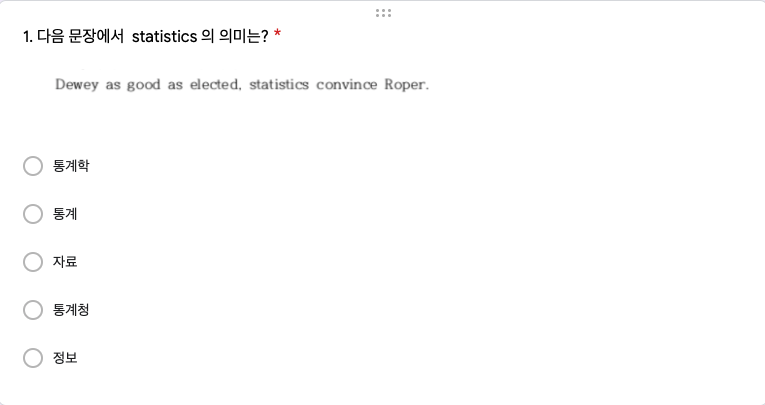
\includegraphics[width=1\linewidth]{./pics/Quiz210302_01} \end{flushleft}

\subsubsection{Roper(Counts)}\label{ropercounts}

\begin{longtable}[]{@{}
  >{\raggedright\arraybackslash}p{(\columnwidth - 12\tabcolsep) * \real{0.1667}}
  >{\centering\arraybackslash}p{(\columnwidth - 12\tabcolsep) * \real{0.1250}}
  >{\centering\arraybackslash}p{(\columnwidth - 12\tabcolsep) * \real{0.0972}}
  >{\centering\arraybackslash}p{(\columnwidth - 12\tabcolsep) * \real{0.0972}}
  >{\centering\arraybackslash}p{(\columnwidth - 12\tabcolsep) * \real{0.1250}}
  >{\centering\arraybackslash}p{(\columnwidth - 12\tabcolsep) * \real{0.0972}}
  >{\centering\arraybackslash}p{(\columnwidth - 12\tabcolsep) * \real{0.0972}}@{}}
\toprule\noalign{}
\begin{minipage}[b]{\linewidth}\raggedright
~
\end{minipage} & \begin{minipage}[b]{\linewidth}\centering
통계학
\end{minipage} & \begin{minipage}[b]{\linewidth}\centering
통계
\end{minipage} & \begin{minipage}[b]{\linewidth}\centering
자료
\end{minipage} & \begin{minipage}[b]{\linewidth}\centering
통계청
\end{minipage} & \begin{minipage}[b]{\linewidth}\centering
정보
\end{minipage} & \begin{minipage}[b]{\linewidth}\centering
계
\end{minipage} \\
\midrule\noalign{}
\endhead
\bottomrule\noalign{}
\endlastfoot
\textbf{Red} & 26 & 230 & 25 & 6 & 5 & 292 \\
\textbf{Black} & 13 & 244 & 14 & 8 & 5 & 284 \\
\textbf{계} & 39 & 474 & 39 & 14 & 10 & 576 \\
\end{longtable}

\begin{longtable}[]{@{}
  >{\raggedleft\arraybackslash}p{(\columnwidth - 4\tabcolsep) * \real{0.2361}}
  >{\raggedleft\arraybackslash}p{(\columnwidth - 4\tabcolsep) * \real{0.0694}}
  >{\raggedleft\arraybackslash}p{(\columnwidth - 4\tabcolsep) * \real{0.1389}}@{}}
\caption{Pearson's Chi-squared test: \texttt{.}}\tabularnewline
\toprule\noalign{}
\begin{minipage}[b]{\linewidth}\raggedleft
Test statistic
\end{minipage} & \begin{minipage}[b]{\linewidth}\raggedleft
df
\end{minipage} & \begin{minipage}[b]{\linewidth}\raggedleft
P value
\end{minipage} \\
\midrule\noalign{}
\endfirsthead
\toprule\noalign{}
\begin{minipage}[b]{\linewidth}\raggedleft
Test statistic
\end{minipage} & \begin{minipage}[b]{\linewidth}\raggedleft
df
\end{minipage} & \begin{minipage}[b]{\linewidth}\raggedleft
P value
\end{minipage} \\
\midrule\noalign{}
\endhead
\bottomrule\noalign{}
\endlastfoot
8.026 & 4 & 0.09065 \\
\end{longtable}

Q1의 집계 결과가 Red, Black 간에 통계적으로 유의한 차이가 있는지
알아보기 위하여 카이제곱 테스트를 수행하였습니다.

그 결과 카이제곱 통계량은 8.03, 자유도는 4, p-value 는 0.0906이므로 Red,
Black 간에 통계적으로 유의한 차이를 보이지 않습니다.

실제로 닮은 게 느껴집니까?

\subsubsection{Roper(\%)}\label{roper}

\begin{longtable}[]{@{}
  >{\centering\arraybackslash}p{(\columnwidth - 10\tabcolsep) * \real{0.1250}}
  >{\centering\arraybackslash}p{(\columnwidth - 10\tabcolsep) * \real{0.0972}}
  >{\centering\arraybackslash}p{(\columnwidth - 10\tabcolsep) * \real{0.0972}}
  >{\centering\arraybackslash}p{(\columnwidth - 10\tabcolsep) * \real{0.1250}}
  >{\centering\arraybackslash}p{(\columnwidth - 10\tabcolsep) * \real{0.0972}}
  >{\centering\arraybackslash}p{(\columnwidth - 10\tabcolsep) * \real{0.1111}}@{}}
\toprule\noalign{}
\begin{minipage}[b]{\linewidth}\centering
통계학
\end{minipage} & \begin{minipage}[b]{\linewidth}\centering
통계
\end{minipage} & \begin{minipage}[b]{\linewidth}\centering
자료
\end{minipage} & \begin{minipage}[b]{\linewidth}\centering
통계청
\end{minipage} & \begin{minipage}[b]{\linewidth}\centering
정보
\end{minipage} & \begin{minipage}[b]{\linewidth}\centering
계
\end{minipage} \\
\midrule\noalign{}
\endhead
\bottomrule\noalign{}
\endlastfoot
6.8 & 82.3 & 6.8 & 2.4 & 1.7 & 100.0 \\
\end{longtable}

정답률은 Red, Black 을 합하여 계산하는데, 82.3(\%) 입니다.

\subsection{Q2. Statistics is the science of learning from data,
\ldots{}}\label{q2.-statistics-is-the-science-of-learning-from-data}

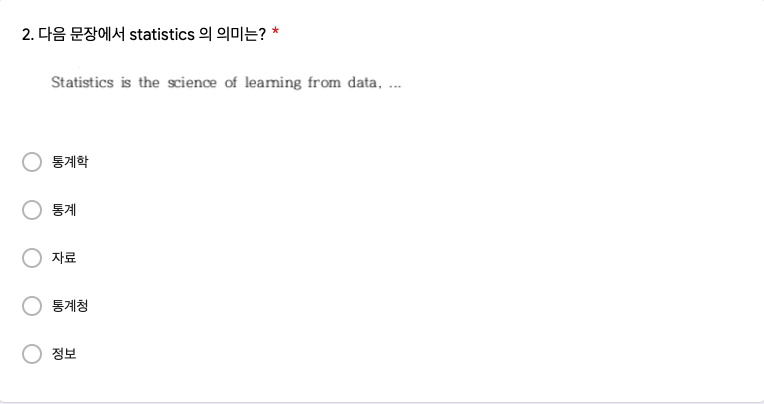
\includegraphics[width=1\linewidth]{./pics/Quiz210302_02}

\subsubsection{ASA(Counts)}\label{asacounts}

\begin{longtable}[]{@{}
  >{\raggedright\arraybackslash}p{(\columnwidth - 12\tabcolsep) * \real{0.1667}}
  >{\centering\arraybackslash}p{(\columnwidth - 12\tabcolsep) * \real{0.1250}}
  >{\centering\arraybackslash}p{(\columnwidth - 12\tabcolsep) * \real{0.0972}}
  >{\centering\arraybackslash}p{(\columnwidth - 12\tabcolsep) * \real{0.0972}}
  >{\centering\arraybackslash}p{(\columnwidth - 12\tabcolsep) * \real{0.1250}}
  >{\centering\arraybackslash}p{(\columnwidth - 12\tabcolsep) * \real{0.0972}}
  >{\centering\arraybackslash}p{(\columnwidth - 12\tabcolsep) * \real{0.0972}}@{}}
\toprule\noalign{}
\begin{minipage}[b]{\linewidth}\raggedright
~
\end{minipage} & \begin{minipage}[b]{\linewidth}\centering
통계학
\end{minipage} & \begin{minipage}[b]{\linewidth}\centering
통계
\end{minipage} & \begin{minipage}[b]{\linewidth}\centering
자료
\end{minipage} & \begin{minipage}[b]{\linewidth}\centering
통계청
\end{minipage} & \begin{minipage}[b]{\linewidth}\centering
정보
\end{minipage} & \begin{minipage}[b]{\linewidth}\centering
계
\end{minipage} \\
\midrule\noalign{}
\endhead
\bottomrule\noalign{}
\endlastfoot
\textbf{Red} & 257 & 27 & 4 & 3 & 1 & 292 \\
\textbf{Black} & 262 & 14 & 3 & 2 & 3 & 284 \\
\textbf{계} & 519 & 41 & 7 & 5 & 4 & 576 \\
\end{longtable}

\begin{longtable}[]{@{}
  >{\raggedleft\arraybackslash}p{(\columnwidth - 4\tabcolsep) * \real{0.2361}}
  >{\raggedleft\arraybackslash}p{(\columnwidth - 4\tabcolsep) * \real{0.0694}}
  >{\raggedleft\arraybackslash}p{(\columnwidth - 4\tabcolsep) * \real{0.1389}}@{}}
\caption{Pearson's Chi-squared test: \texttt{.}}\tabularnewline
\toprule\noalign{}
\begin{minipage}[b]{\linewidth}\raggedleft
Test statistic
\end{minipage} & \begin{minipage}[b]{\linewidth}\raggedleft
df
\end{minipage} & \begin{minipage}[b]{\linewidth}\raggedleft
P value
\end{minipage} \\
\midrule\noalign{}
\endfirsthead
\toprule\noalign{}
\begin{minipage}[b]{\linewidth}\raggedleft
Test statistic
\end{minipage} & \begin{minipage}[b]{\linewidth}\raggedleft
df
\end{minipage} & \begin{minipage}[b]{\linewidth}\raggedleft
P value
\end{minipage} \\
\midrule\noalign{}
\endhead
\bottomrule\noalign{}
\endlastfoot
5.403 & 4 & 0.2484 \\
\end{longtable}

Q2의 집계 결과가 Red, Black 간에 통계적으로 유의한 차이가 있는지
알아보기 위하여 카이제곱 테스트를 수행하였습니다.

그 결과 카이제곱 통계량은 5.403, 자유도는 4, p-value 는 0.2484이므로
Red, Black 간에 통계적으로 유의한 차이를 보이지 않습니다.

실제로 닮은 게 느껴집니까?

\subsubsection{ASA(\%)}\label{asa}

\begin{longtable}[]{@{}
  >{\centering\arraybackslash}p{(\columnwidth - 10\tabcolsep) * \real{0.1250}}
  >{\centering\arraybackslash}p{(\columnwidth - 10\tabcolsep) * \real{0.0972}}
  >{\centering\arraybackslash}p{(\columnwidth - 10\tabcolsep) * \real{0.0972}}
  >{\centering\arraybackslash}p{(\columnwidth - 10\tabcolsep) * \real{0.1250}}
  >{\centering\arraybackslash}p{(\columnwidth - 10\tabcolsep) * \real{0.0972}}
  >{\centering\arraybackslash}p{(\columnwidth - 10\tabcolsep) * \real{0.1250}}@{}}
\toprule\noalign{}
\begin{minipage}[b]{\linewidth}\centering
통계학
\end{minipage} & \begin{minipage}[b]{\linewidth}\centering
통계
\end{minipage} & \begin{minipage}[b]{\linewidth}\centering
자료
\end{minipage} & \begin{minipage}[b]{\linewidth}\centering
통계청
\end{minipage} & \begin{minipage}[b]{\linewidth}\centering
정보
\end{minipage} & \begin{minipage}[b]{\linewidth}\centering
계
\end{minipage} \\
\midrule\noalign{}
\endhead
\bottomrule\noalign{}
\endlastfoot
90.10 & 7.12 & 1.22 & 0.87 & 0.69 & 100.00 \\
\end{longtable}

정답률은 Red, Black 을 합하여 계산하는데, 90.1(\%) 입니다.

\subsection{Q3. How to lie with
statistics}\label{q3.-how-to-lie-with-statistics}

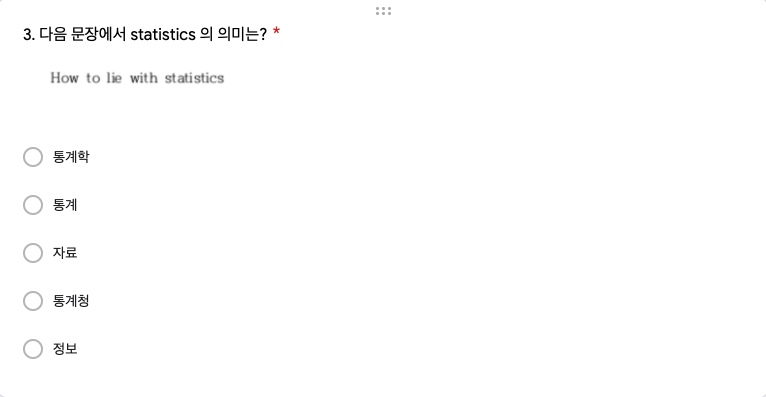
\includegraphics[width=1\linewidth]{./pics/Quiz210302_03}

\subsubsection{D.Huff(Counts)}\label{d.huffcounts}

\begin{longtable}[]{@{}
  >{\raggedright\arraybackslash}p{(\columnwidth - 12\tabcolsep) * \real{0.1667}}
  >{\centering\arraybackslash}p{(\columnwidth - 12\tabcolsep) * \real{0.1250}}
  >{\centering\arraybackslash}p{(\columnwidth - 12\tabcolsep) * \real{0.0972}}
  >{\centering\arraybackslash}p{(\columnwidth - 12\tabcolsep) * \real{0.0972}}
  >{\centering\arraybackslash}p{(\columnwidth - 12\tabcolsep) * \real{0.1250}}
  >{\centering\arraybackslash}p{(\columnwidth - 12\tabcolsep) * \real{0.0972}}
  >{\centering\arraybackslash}p{(\columnwidth - 12\tabcolsep) * \real{0.0972}}@{}}
\toprule\noalign{}
\begin{minipage}[b]{\linewidth}\raggedright
~
\end{minipage} & \begin{minipage}[b]{\linewidth}\centering
통계학
\end{minipage} & \begin{minipage}[b]{\linewidth}\centering
통계
\end{minipage} & \begin{minipage}[b]{\linewidth}\centering
자료
\end{minipage} & \begin{minipage}[b]{\linewidth}\centering
통계청
\end{minipage} & \begin{minipage}[b]{\linewidth}\centering
정보
\end{minipage} & \begin{minipage}[b]{\linewidth}\centering
계
\end{minipage} \\
\midrule\noalign{}
\endhead
\bottomrule\noalign{}
\endlastfoot
\textbf{Red} & 14 & 204 & 41 & 14 & 19 & 292 \\
\textbf{Black} & 16 & 213 & 28 & 6 & 21 & 284 \\
\textbf{계} & 30 & 417 & 69 & 20 & 40 & 576 \\
\end{longtable}

\begin{longtable}[]{@{}
  >{\raggedleft\arraybackslash}p{(\columnwidth - 4\tabcolsep) * \real{0.2361}}
  >{\raggedleft\arraybackslash}p{(\columnwidth - 4\tabcolsep) * \real{0.0694}}
  >{\raggedleft\arraybackslash}p{(\columnwidth - 4\tabcolsep) * \real{0.1389}}@{}}
\caption{Pearson's Chi-squared test: \texttt{.}}\tabularnewline
\toprule\noalign{}
\begin{minipage}[b]{\linewidth}\raggedleft
Test statistic
\end{minipage} & \begin{minipage}[b]{\linewidth}\raggedleft
df
\end{minipage} & \begin{minipage}[b]{\linewidth}\raggedleft
P value
\end{minipage} \\
\midrule\noalign{}
\endfirsthead
\toprule\noalign{}
\begin{minipage}[b]{\linewidth}\raggedleft
Test statistic
\end{minipage} & \begin{minipage}[b]{\linewidth}\raggedleft
df
\end{minipage} & \begin{minipage}[b]{\linewidth}\raggedleft
P value
\end{minipage} \\
\midrule\noalign{}
\endhead
\bottomrule\noalign{}
\endlastfoot
5.967 & 4 & 0.2016 \\
\end{longtable}

Q3의 집계 결과가 Red, Black 간에 통계적으로 유의한 차이가 있는지
알아보기 위하여 카이제곱 테스트를 수행하였습니다.

그 결과 카이제곱 통계량은 5.967, 자유도는 4, p-value 는 0.2016이므로
Red, Black 간에 통계적으로 유의한 차이를 보이지 않습니다.

실제로 닮은 게 느껴집니까?

\subsubsection{D.Huff(\%)}\label{d.huff}

\begin{longtable}[]{@{}
  >{\centering\arraybackslash}p{(\columnwidth - 10\tabcolsep) * \real{0.1250}}
  >{\centering\arraybackslash}p{(\columnwidth - 10\tabcolsep) * \real{0.0972}}
  >{\centering\arraybackslash}p{(\columnwidth - 10\tabcolsep) * \real{0.0972}}
  >{\centering\arraybackslash}p{(\columnwidth - 10\tabcolsep) * \real{0.1250}}
  >{\centering\arraybackslash}p{(\columnwidth - 10\tabcolsep) * \real{0.0972}}
  >{\centering\arraybackslash}p{(\columnwidth - 10\tabcolsep) * \real{0.1111}}@{}}
\toprule\noalign{}
\begin{minipage}[b]{\linewidth}\centering
통계학
\end{minipage} & \begin{minipage}[b]{\linewidth}\centering
통계
\end{minipage} & \begin{minipage}[b]{\linewidth}\centering
자료
\end{minipage} & \begin{minipage}[b]{\linewidth}\centering
통계청
\end{minipage} & \begin{minipage}[b]{\linewidth}\centering
정보
\end{minipage} & \begin{minipage}[b]{\linewidth}\centering
계
\end{minipage} \\
\midrule\noalign{}
\endhead
\bottomrule\noalign{}
\endlastfoot
5.2 & 72.4 & 12.0 & 3.5 & 6.9 & 100.0 \\
\end{longtable}

정답률은 Red, Black 을 합하여 계산하는데, 72.4(\%) 입니다.

\subsection{Q4. 종부세}\label{q4.-uxc885uxbd80uxc138}

``바람직한 논의이다''라는 선택지에 부연설명을 붙이거나(Red), ``부적절한
논의이다''라는 선택지에 부연설명을 붙였을 때(Black), 부연설명의 여부에
따라 응답이 달라지는 지 살펴본 결과 기대와는 달리 통계적으로 유의한
수준의 차이를 관찰하지 못하였습니다.

앞에서 본 바와 같이 Red, Black 두 집단은 출석부의 다섯 변수에 대하여
랜덤화 과정을 거쳐서 가장 닮은 구성을 찾은 것이기에 Q1, Q2, Q3의 응답
결과도 매우 닮게 나오는데 만약 부연설명이 효과가 없다면 Q4에서의 응답도
닮게 나왔을 것입니다.

지난 학기들과 달리 통계적으로 유의한 차이를 관찰하지 못한 이유를 따져 볼
필요가 있겠습니다.

\subsubsection{질문지 선택지에
부연설명}\label{uxc9c8uxbb38uxc9c0-uxc120uxd0dduxc9c0uxc5d0-uxbd80uxc5f0uxc124uxba85}

\begin{flushleft}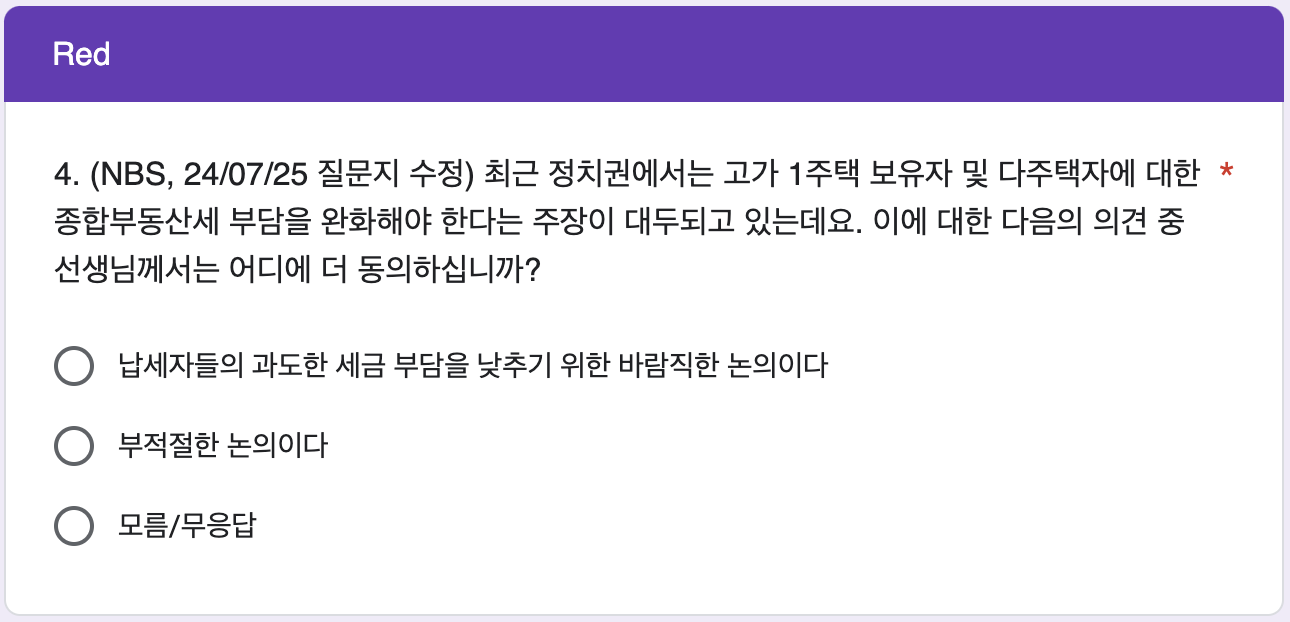
\includegraphics[width=0.67\linewidth]{./pics/Quiz240902_Q4_Red} \end{flushleft}

\begin{flushleft}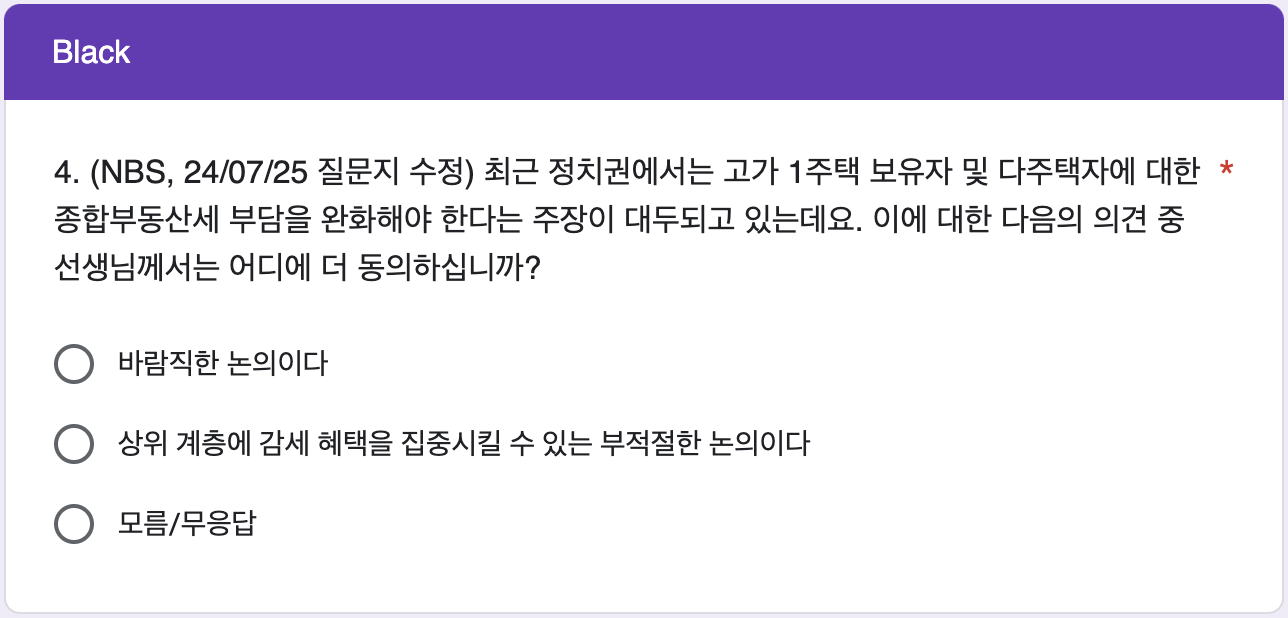
\includegraphics[width=0.67\linewidth]{./pics/Quiz240902_Q4_Black} \end{flushleft}

\subsubsection{집계}\label{uxc9d1uxacc4}

\begin{longtable}[]{@{}
  >{\raggedright\arraybackslash}p{(\columnwidth - 8\tabcolsep) * \real{0.3023}}
  >{\centering\arraybackslash}p{(\columnwidth - 8\tabcolsep) * \real{0.2326}}
  >{\centering\arraybackslash}p{(\columnwidth - 8\tabcolsep) * \real{0.2326}}
  >{\centering\arraybackslash}p{(\columnwidth - 8\tabcolsep) * \real{0.1628}}
  >{\centering\arraybackslash}p{(\columnwidth - 8\tabcolsep) * \real{0.0698}}@{}}
\toprule\noalign{}
\begin{minipage}[b]{\linewidth}\raggedright
~
\end{minipage} & \begin{minipage}[b]{\linewidth}\centering
바람직한 논의이다
\end{minipage} & \begin{minipage}[b]{\linewidth}\centering
부적절한 논의이다
\end{minipage} & \begin{minipage}[b]{\linewidth}\centering
모름/무응답
\end{minipage} & \begin{minipage}[b]{\linewidth}\centering
계
\end{minipage} \\
\midrule\noalign{}
\endhead
\bottomrule\noalign{}
\endlastfoot
\textbf{Red(바람직한 논의에 부연설명)} & 95 & 113 & 84 & 292 \\
\textbf{Black(부적절한 논의에 부연설명)} & 72 & 130 & 82 & 284 \\
\textbf{계} & 167 & 243 & 166 & 576 \\
\end{longtable}

\begin{longtable}[]{@{}
  >{\raggedleft\arraybackslash}p{(\columnwidth - 4\tabcolsep) * \real{0.2361}}
  >{\raggedleft\arraybackslash}p{(\columnwidth - 4\tabcolsep) * \real{0.0694}}
  >{\raggedleft\arraybackslash}p{(\columnwidth - 4\tabcolsep) * \real{0.1389}}@{}}
\caption{Pearson's Chi-squared test: \texttt{.}}\tabularnewline
\toprule\noalign{}
\begin{minipage}[b]{\linewidth}\raggedleft
Test statistic
\end{minipage} & \begin{minipage}[b]{\linewidth}\raggedleft
df
\end{minipage} & \begin{minipage}[b]{\linewidth}\raggedleft
P value
\end{minipage} \\
\midrule\noalign{}
\endfirsthead
\toprule\noalign{}
\begin{minipage}[b]{\linewidth}\raggedleft
Test statistic
\end{minipage} & \begin{minipage}[b]{\linewidth}\raggedleft
df
\end{minipage} & \begin{minipage}[b]{\linewidth}\raggedleft
P value
\end{minipage} \\
\midrule\noalign{}
\endhead
\bottomrule\noalign{}
\endlastfoot
4.271 & 2 & 0.1182 \\
\end{longtable}

Q4의 Red에는 종합부동산세 부담을 완화해야 한다는 주장에 대하여 바람직한
논의라는 쪽에 긍정적인 부연설명을 붙였는데, 292명이 응답한 가운데 95명이
``바람직한 논의이다''라는 반응을 보이고, 113명이 ``부적절한
논의이다''라는 반응을 보입니다.

Black에는 같은 주장에 대하여 부적절한 논의라는 쪽에 부정적인 부연설명을
붙였는데, 284명이 응답한 가운데 72명이 ``바람직한 논의이다''라는 반응을
보이고, 130명이 ``부적절한 논의이다''라는 반응을 보입니다.

그리고 ``모름/무응답''에 답한 인원은 Red에 84명, Black 에 82명이
응답하였습니다.

지난 학기 자료들에서 볼 수 있다시피 카이제곱 테스트는 이와 같은 상황에서
부연설명의 유무가 응답에 미치는 영향이 대부분 통계적으로 유의하다는 것을
보여 줍니다.

그런데, 이번 학기는 매우 예외적으로 그렇지 않은 경우가 관찰되었습니다.

카이제곱 통계량은 4.271, 자유도는 2, p-value 는 0.1182으로 부연설명을
어떻게 붙이느냐에 따라 반응이 다르게 나온다는 것을 보여주고 싶었지만
실제로 관찰된 차이는 Q1 \textasciitilde{} Q3와 마찬가지로 통계적으로
유의한 수준은 아닙니다.

여기서 부연설명이 응답에 영향을 끼치지 않는다고 가정해 봅시다.

그렇다면 Red, Black 의 응답은 Q1\textasciitilde Q3 에서와 같이 랜덤화
효과에 의하여 통계적으로 유의한 차이를 보이지 않을 것입니다.

그런데 실제로 관찰된 카이제곱 통계값과 P-value 는 통계적으로 유의한
차이를 보여 주지 못하는 수준입니다.

따라서 부연설명이 영향을 끼치지 않는다는 가정을 받아들일 수밖에 없게
되었습니다.

지난 학기 자료들이 모두 통계적으로 유의한 차이를 보여 주었던 것과는 달리
이번 학기에 유독 통계적으로 유의한 차이를 보이지 않는 이유는 무엇일까요?

\subsubsection{\% 비교.}\label{uxbe44uxad50.}

\begin{longtable}[]{@{}
  >{\raggedright\arraybackslash}p{(\columnwidth - 8\tabcolsep) * \real{0.2955}}
  >{\centering\arraybackslash}p{(\columnwidth - 8\tabcolsep) * \real{0.2273}}
  >{\centering\arraybackslash}p{(\columnwidth - 8\tabcolsep) * \real{0.2273}}
  >{\centering\arraybackslash}p{(\columnwidth - 8\tabcolsep) * \real{0.1591}}
  >{\centering\arraybackslash}p{(\columnwidth - 8\tabcolsep) * \real{0.0909}}@{}}
\toprule\noalign{}
\begin{minipage}[b]{\linewidth}\raggedright
~
\end{minipage} & \begin{minipage}[b]{\linewidth}\centering
바람직한 논의이다
\end{minipage} & \begin{minipage}[b]{\linewidth}\centering
부적절한 논의이다
\end{minipage} & \begin{minipage}[b]{\linewidth}\centering
모름/무응답
\end{minipage} & \begin{minipage}[b]{\linewidth}\centering
계
\end{minipage} \\
\midrule\noalign{}
\endhead
\bottomrule\noalign{}
\endlastfoot
\textbf{Red(바람직한 논의에 부연설명)} & 32.5 & 38.7 & 28.8 & 100.0 \\
\textbf{Black(부적절한 논의에 부연설명)} & 25.4 & 45.8 & 28.9 & 100.0 \\
\end{longtable}

``바람직한 논의이다''에 부연설명을 붙인 Red에서 ``바람직한
논의이다''라고 응답하는 사람들의 백분율, 32.5(\%)은 ``부적절한
논의이다''에 부연설명을 붙인 Black 에서 ``바람직한 논의이다''라고
응답하는 사람들의 백분율, 25.4(\%) 보다 높습니다.

반면 ``부적절한 논의이다''에 부연설명을 붙인 Black 에서 ``부적절한
논의이다''라고 응답하는 사람들의 백분율, 45.8(\%)은 Red 에서 ``부적절한
논의이다''라고 응답하는 사람들의 백분율, 38.7(\%) 보다 높습니다.

부연설명을 어디에 붙이느냐에 따라 반응이 치우치는 것을 알 수 있지만
p-value 가 보여주듯이 \textbf{그 차이가 통계적으로 유의한 수준은 아닌
것}입니다.

\subsubsection{Mosaic Plot}\label{mosaic-plot}

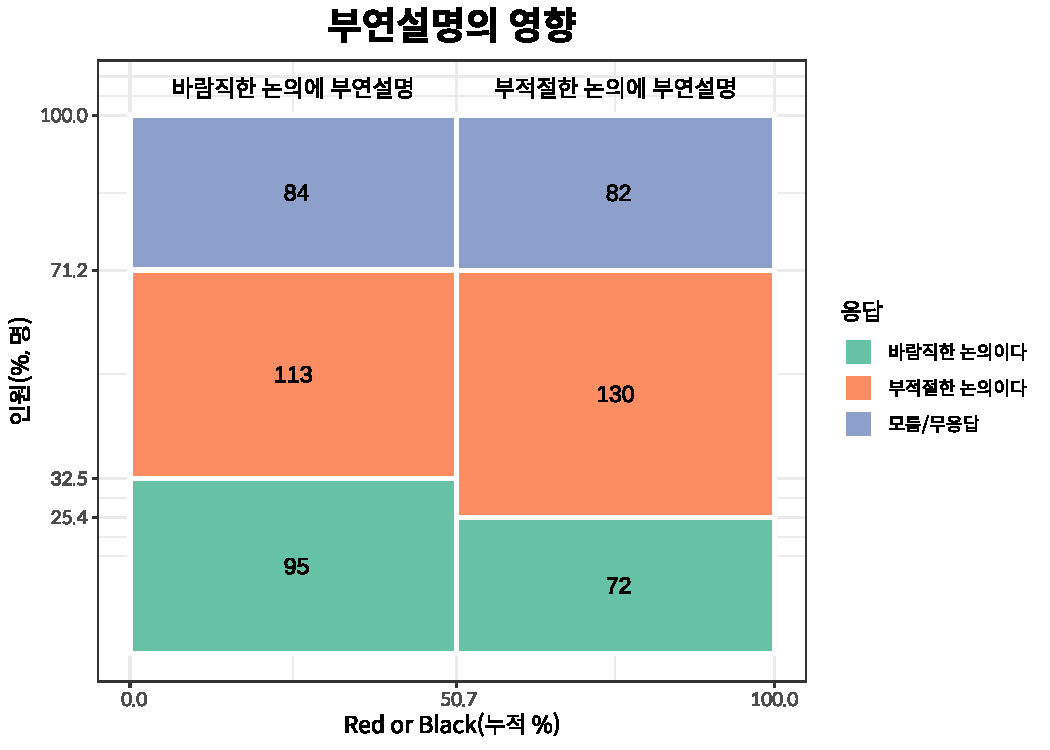
\includegraphics{quiz250303_Report_v7_files/figure-latex/mosaic plot-1.pdf}

Mosaic Plot 은 이 집계결과를 시각적으로 잘 보여줍니다.

``바람직한 논의이다''에 부연설명을 붙인 Red 에서 ``바람직힌
논의이다''라고 응답한 백분율이 ``부적절한 논의이다''에 부연설명을 붙인
Black 에서 ``바람직한 논의이다''라고 응답한 백분율보다 높고, Black 에서
``부적절한 논의이다''라고 응답한 백분율은 Red 에서 ``부적절한
논의이다''라고 응답한 백분율보다 월등히 높습니다.

\subsection{마감 시간으로부터 제출 시간의
분포}\label{uxb9c8uxac10-uxc2dcuxac04uxc73cuxb85cuxbd80uxd130-uxc81cuxcd9c-uxc2dcuxac04uxc758-uxbd84uxd3ec}

\subsubsection{분포표}\label{uxbd84uxd3ecuxd45c}

\begin{longtable}[]{@{}
  >{\raggedright\arraybackslash}p{(\columnwidth - 30\tabcolsep) * \real{0.0863}}
  >{\raggedleft\arraybackslash}p{(\columnwidth - 30\tabcolsep) * \real{0.0576}}
  >{\raggedleft\arraybackslash}p{(\columnwidth - 30\tabcolsep) * \real{0.0576}}
  >{\raggedleft\arraybackslash}p{(\columnwidth - 30\tabcolsep) * \real{0.0576}}
  >{\raggedleft\arraybackslash}p{(\columnwidth - 30\tabcolsep) * \real{0.0576}}
  >{\raggedleft\arraybackslash}p{(\columnwidth - 30\tabcolsep) * \real{0.0576}}
  >{\raggedleft\arraybackslash}p{(\columnwidth - 30\tabcolsep) * \real{0.0576}}
  >{\raggedleft\arraybackslash}p{(\columnwidth - 30\tabcolsep) * \real{0.0576}}
  >{\raggedleft\arraybackslash}p{(\columnwidth - 30\tabcolsep) * \real{0.0576}}
  >{\raggedleft\arraybackslash}p{(\columnwidth - 30\tabcolsep) * \real{0.0576}}
  >{\raggedleft\arraybackslash}p{(\columnwidth - 30\tabcolsep) * \real{0.0647}}
  >{\raggedleft\arraybackslash}p{(\columnwidth - 30\tabcolsep) * \real{0.0719}}
  >{\raggedleft\arraybackslash}p{(\columnwidth - 30\tabcolsep) * \real{0.0719}}
  >{\raggedleft\arraybackslash}p{(\columnwidth - 30\tabcolsep) * \real{0.0719}}
  >{\raggedleft\arraybackslash}p{(\columnwidth - 30\tabcolsep) * \real{0.0719}}
  >{\centering\arraybackslash}p{(\columnwidth - 30\tabcolsep) * \real{0.0432}}@{}}
\caption{일 단위}\tabularnewline
\toprule\noalign{}
\begin{minipage}[b]{\linewidth}\raggedright
~
\end{minipage} & \begin{minipage}[b]{\linewidth}\raggedleft
{[}0,1{]}
\end{minipage} & \begin{minipage}[b]{\linewidth}\raggedleft
(1,2{]}
\end{minipage} & \begin{minipage}[b]{\linewidth}\raggedleft
(2,3{]}
\end{minipage} & \begin{minipage}[b]{\linewidth}\raggedleft
(3,4{]}
\end{minipage} & \begin{minipage}[b]{\linewidth}\raggedleft
(4,5{]}
\end{minipage} & \begin{minipage}[b]{\linewidth}\raggedleft
(5,6{]}
\end{minipage} & \begin{minipage}[b]{\linewidth}\raggedleft
(6,7{]}
\end{minipage} & \begin{minipage}[b]{\linewidth}\raggedleft
(7,8{]}
\end{minipage} & \begin{minipage}[b]{\linewidth}\raggedleft
(8,9{]}
\end{minipage} & \begin{minipage}[b]{\linewidth}\raggedleft
(9,10{]}
\end{minipage} & \begin{minipage}[b]{\linewidth}\raggedleft
(10,11{]}
\end{minipage} & \begin{minipage}[b]{\linewidth}\raggedleft
(11,12{]}
\end{minipage} & \begin{minipage}[b]{\linewidth}\raggedleft
(12,13{]}
\end{minipage} & \begin{minipage}[b]{\linewidth}\raggedleft
(13,14{]}
\end{minipage} & \begin{minipage}[b]{\linewidth}\centering
계
\end{minipage} \\
\midrule\noalign{}
\endfirsthead
\toprule\noalign{}
\begin{minipage}[b]{\linewidth}\raggedright
~
\end{minipage} & \begin{minipage}[b]{\linewidth}\raggedleft
{[}0,1{]}
\end{minipage} & \begin{minipage}[b]{\linewidth}\raggedleft
(1,2{]}
\end{minipage} & \begin{minipage}[b]{\linewidth}\raggedleft
(2,3{]}
\end{minipage} & \begin{minipage}[b]{\linewidth}\raggedleft
(3,4{]}
\end{minipage} & \begin{minipage}[b]{\linewidth}\raggedleft
(4,5{]}
\end{minipage} & \begin{minipage}[b]{\linewidth}\raggedleft
(5,6{]}
\end{minipage} & \begin{minipage}[b]{\linewidth}\raggedleft
(6,7{]}
\end{minipage} & \begin{minipage}[b]{\linewidth}\raggedleft
(7,8{]}
\end{minipage} & \begin{minipage}[b]{\linewidth}\raggedleft
(8,9{]}
\end{minipage} & \begin{minipage}[b]{\linewidth}\raggedleft
(9,10{]}
\end{minipage} & \begin{minipage}[b]{\linewidth}\raggedleft
(10,11{]}
\end{minipage} & \begin{minipage}[b]{\linewidth}\raggedleft
(11,12{]}
\end{minipage} & \begin{minipage}[b]{\linewidth}\raggedleft
(12,13{]}
\end{minipage} & \begin{minipage}[b]{\linewidth}\raggedleft
(13,14{]}
\end{minipage} & \begin{minipage}[b]{\linewidth}\centering
계
\end{minipage} \\
\midrule\noalign{}
\endhead
\bottomrule\noalign{}
\endlastfoot
\textbf{Red} & 46 & 11 & 6 & 11 & 6 & 14 & 10 & 42 & 21 & 19 & 15 & 30 &
35 & 26 & 292 \\
\textbf{Black} & 35 & 10 & 6 & 7 & 5 & 12 & 12 & 34 & 22 & 17 & 26 & 37
& 29 & 32 & 284 \\
\textbf{계} & 81 & 21 & 12 & 18 & 11 & 26 & 22 & 76 & 43 & 36 & 41 & 67
& 64 & 58 & 576 \\
\end{longtable}

분포표로부터 두 가지 문제를 살펴보겠습니다.

첫째, 날마다 고르게 제출하는가?

둘째, Red, Black 간에 통계적으로 유의한 차이가 있는가?

각 문제를 살펴보기 위해서는 분포표의 일부분을 대상으로 카이제곱 테스트를
수행합니다.

\subsubsection{날마다 고르게
제출하는가?}\label{uxb0a0uxb9c8uxb2e4-uxace0uxb974uxac8c-uxc81cuxcd9cuxd558uxb294uxac00}

\begin{longtable}[]{@{}
  >{\raggedleft\arraybackslash}p{(\columnwidth - 26\tabcolsep) * \real{0.0661}}
  >{\raggedleft\arraybackslash}p{(\columnwidth - 26\tabcolsep) * \real{0.0661}}
  >{\raggedleft\arraybackslash}p{(\columnwidth - 26\tabcolsep) * \real{0.0661}}
  >{\raggedleft\arraybackslash}p{(\columnwidth - 26\tabcolsep) * \real{0.0661}}
  >{\raggedleft\arraybackslash}p{(\columnwidth - 26\tabcolsep) * \real{0.0661}}
  >{\raggedleft\arraybackslash}p{(\columnwidth - 26\tabcolsep) * \real{0.0661}}
  >{\raggedleft\arraybackslash}p{(\columnwidth - 26\tabcolsep) * \real{0.0661}}
  >{\raggedleft\arraybackslash}p{(\columnwidth - 26\tabcolsep) * \real{0.0661}}
  >{\raggedleft\arraybackslash}p{(\columnwidth - 26\tabcolsep) * \real{0.0661}}
  >{\raggedleft\arraybackslash}p{(\columnwidth - 26\tabcolsep) * \real{0.0744}}
  >{\raggedleft\arraybackslash}p{(\columnwidth - 26\tabcolsep) * \real{0.0826}}
  >{\raggedleft\arraybackslash}p{(\columnwidth - 26\tabcolsep) * \real{0.0826}}
  >{\raggedleft\arraybackslash}p{(\columnwidth - 26\tabcolsep) * \real{0.0826}}
  >{\raggedleft\arraybackslash}p{(\columnwidth - 26\tabcolsep) * \real{0.0826}}@{}}
\toprule\noalign{}
\begin{minipage}[b]{\linewidth}\raggedleft
{[}0,1{]}
\end{minipage} & \begin{minipage}[b]{\linewidth}\raggedleft
(1,2{]}
\end{minipage} & \begin{minipage}[b]{\linewidth}\raggedleft
(2,3{]}
\end{minipage} & \begin{minipage}[b]{\linewidth}\raggedleft
(3,4{]}
\end{minipage} & \begin{minipage}[b]{\linewidth}\raggedleft
(4,5{]}
\end{minipage} & \begin{minipage}[b]{\linewidth}\raggedleft
(5,6{]}
\end{minipage} & \begin{minipage}[b]{\linewidth}\raggedleft
(6,7{]}
\end{minipage} & \begin{minipage}[b]{\linewidth}\raggedleft
(7,8{]}
\end{minipage} & \begin{minipage}[b]{\linewidth}\raggedleft
(8,9{]}
\end{minipage} & \begin{minipage}[b]{\linewidth}\raggedleft
(9,10{]}
\end{minipage} & \begin{minipage}[b]{\linewidth}\raggedleft
(10,11{]}
\end{minipage} & \begin{minipage}[b]{\linewidth}\raggedleft
(11,12{]}
\end{minipage} & \begin{minipage}[b]{\linewidth}\raggedleft
(12,13{]}
\end{minipage} & \begin{minipage}[b]{\linewidth}\raggedleft
(13,14{]}
\end{minipage} \\
\midrule\noalign{}
\endhead
\bottomrule\noalign{}
\endlastfoot
81 & 21 & 12 & 18 & 11 & 26 & 22 & 76 & 43 & 36 & 41 & 67 & 64 & 58 \\
\end{longtable}

\begin{longtable}[]{@{}
  >{\raggedleft\arraybackslash}p{(\columnwidth - 4\tabcolsep) * \real{0.2361}}
  >{\raggedleft\arraybackslash}p{(\columnwidth - 4\tabcolsep) * \real{0.0694}}
  >{\raggedleft\arraybackslash}p{(\columnwidth - 4\tabcolsep) * \real{0.2500}}@{}}
\caption{Chi-squared test for given probabilities:
\texttt{.}}\tabularnewline
\toprule\noalign{}
\begin{minipage}[b]{\linewidth}\raggedleft
Test statistic
\end{minipage} & \begin{minipage}[b]{\linewidth}\raggedleft
df
\end{minipage} & \begin{minipage}[b]{\linewidth}\raggedleft
P value
\end{minipage} \\
\midrule\noalign{}
\endfirsthead
\toprule\noalign{}
\begin{minipage}[b]{\linewidth}\raggedleft
Test statistic
\end{minipage} & \begin{minipage}[b]{\linewidth}\raggedleft
df
\end{minipage} & \begin{minipage}[b]{\linewidth}\raggedleft
P value
\end{minipage} \\
\midrule\noalign{}
\endhead
\bottomrule\noalign{}
\endlastfoot
184.8 & 13 & 1.766e-32 * * * \\
\end{longtable}

날마다 고르게 제출하는지 알아 보았습니다.

분포표의 ``계''행에서 '계'열을 제외하고 카이제곱테스트를 수행합니다.

분포표 만으로도 쉽게 파악할 수 있지만 카이제곱테스트가 명확히 해 줍니다.

카이제곱 통계량은 184.812, 자유도는 13, p-value 는 1.8e-32 이므로 결코
고르게 제출한다고 말할 수 없겠습니다.

막대그래프로 살펴 보겠습니다.

\subsubsection{막대그래프}\label{uxb9c9uxb300uxadf8uxb798uxd504}

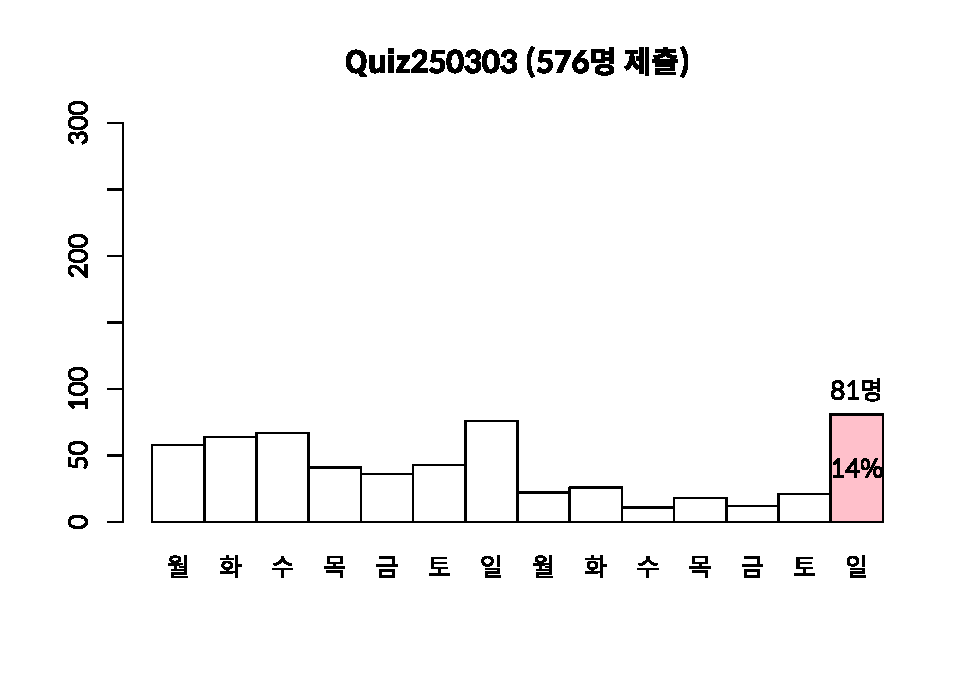
\includegraphics{quiz250303_Report_v7_files/figure-latex/unnamed-chunk-8-1.pdf}

막대그래프는 총 제출인원 576(명) 중에 81(명), 14(\%)가 마감일에 몰리는
것을 보여주고 있습니다.

\subsubsection{Red, Black 간에
닮았는가?}\label{red-black-uxac04uxc5d0-uxb2eeuxc558uxb294uxac00}

\begin{longtable}[]{@{}
  >{\raggedright\arraybackslash}p{(\columnwidth - 28\tabcolsep) * \real{0.0902}}
  >{\raggedleft\arraybackslash}p{(\columnwidth - 28\tabcolsep) * \real{0.0602}}
  >{\raggedleft\arraybackslash}p{(\columnwidth - 28\tabcolsep) * \real{0.0602}}
  >{\raggedleft\arraybackslash}p{(\columnwidth - 28\tabcolsep) * \real{0.0602}}
  >{\raggedleft\arraybackslash}p{(\columnwidth - 28\tabcolsep) * \real{0.0602}}
  >{\raggedleft\arraybackslash}p{(\columnwidth - 28\tabcolsep) * \real{0.0602}}
  >{\raggedleft\arraybackslash}p{(\columnwidth - 28\tabcolsep) * \real{0.0602}}
  >{\raggedleft\arraybackslash}p{(\columnwidth - 28\tabcolsep) * \real{0.0602}}
  >{\raggedleft\arraybackslash}p{(\columnwidth - 28\tabcolsep) * \real{0.0602}}
  >{\raggedleft\arraybackslash}p{(\columnwidth - 28\tabcolsep) * \real{0.0602}}
  >{\raggedleft\arraybackslash}p{(\columnwidth - 28\tabcolsep) * \real{0.0677}}
  >{\raggedleft\arraybackslash}p{(\columnwidth - 28\tabcolsep) * \real{0.0752}}
  >{\raggedleft\arraybackslash}p{(\columnwidth - 28\tabcolsep) * \real{0.0752}}
  >{\raggedleft\arraybackslash}p{(\columnwidth - 28\tabcolsep) * \real{0.0752}}
  >{\raggedleft\arraybackslash}p{(\columnwidth - 28\tabcolsep) * \real{0.0752}}@{}}
\toprule\noalign{}
\begin{minipage}[b]{\linewidth}\raggedright
~
\end{minipage} & \begin{minipage}[b]{\linewidth}\raggedleft
{[}0,1{]}
\end{minipage} & \begin{minipage}[b]{\linewidth}\raggedleft
(1,2{]}
\end{minipage} & \begin{minipage}[b]{\linewidth}\raggedleft
(2,3{]}
\end{minipage} & \begin{minipage}[b]{\linewidth}\raggedleft
(3,4{]}
\end{minipage} & \begin{minipage}[b]{\linewidth}\raggedleft
(4,5{]}
\end{minipage} & \begin{minipage}[b]{\linewidth}\raggedleft
(5,6{]}
\end{minipage} & \begin{minipage}[b]{\linewidth}\raggedleft
(6,7{]}
\end{minipage} & \begin{minipage}[b]{\linewidth}\raggedleft
(7,8{]}
\end{minipage} & \begin{minipage}[b]{\linewidth}\raggedleft
(8,9{]}
\end{minipage} & \begin{minipage}[b]{\linewidth}\raggedleft
(9,10{]}
\end{minipage} & \begin{minipage}[b]{\linewidth}\raggedleft
(10,11{]}
\end{minipage} & \begin{minipage}[b]{\linewidth}\raggedleft
(11,12{]}
\end{minipage} & \begin{minipage}[b]{\linewidth}\raggedleft
(12,13{]}
\end{minipage} & \begin{minipage}[b]{\linewidth}\raggedleft
(13,14{]}
\end{minipage} \\
\midrule\noalign{}
\endhead
\bottomrule\noalign{}
\endlastfoot
\textbf{Red} & 46 & 11 & 6 & 11 & 6 & 14 & 10 & 42 & 21 & 19 & 15 & 30 &
35 & 26 \\
\textbf{Black} & 35 & 10 & 6 & 7 & 5 & 12 & 12 & 34 & 22 & 17 & 26 & 37
& 29 & 32 \\
\end{longtable}

\begin{longtable}[]{@{}
  >{\raggedleft\arraybackslash}p{(\columnwidth - 4\tabcolsep) * \real{0.2361}}
  >{\raggedleft\arraybackslash}p{(\columnwidth - 4\tabcolsep) * \real{0.0694}}
  >{\raggedleft\arraybackslash}p{(\columnwidth - 4\tabcolsep) * \real{0.1389}}@{}}
\caption{Pearson's Chi-squared test: \texttt{.}}\tabularnewline
\toprule\noalign{}
\begin{minipage}[b]{\linewidth}\raggedleft
Test statistic
\end{minipage} & \begin{minipage}[b]{\linewidth}\raggedleft
df
\end{minipage} & \begin{minipage}[b]{\linewidth}\raggedleft
P value
\end{minipage} \\
\midrule\noalign{}
\endfirsthead
\toprule\noalign{}
\begin{minipage}[b]{\linewidth}\raggedleft
Test statistic
\end{minipage} & \begin{minipage}[b]{\linewidth}\raggedleft
df
\end{minipage} & \begin{minipage}[b]{\linewidth}\raggedleft
P value
\end{minipage} \\
\midrule\noalign{}
\endhead
\bottomrule\noalign{}
\endlastfoot
8.59 & 13 & 0.8032 \\
\end{longtable}

제출시간의 분포가 Red, Black 간에 닮았는지 알아 보았습니다.

이번에는 분포표의 첫번째와 두번째 행, '계'열을 제외한 나머지 열에 대해서
카이제곱테스트를 수행합니다.

카이제곱 통계량은 8.590, 자유도는 13, p-value 는 0.8032 이므로 제출
시간의 분포는 Red, Black 간에 통계적으로 유의한 차이가 관찰되지
않습니다.

이 사실을 Mosaic Plot 을 이용하여 시각적으로 살펴보겠습니다.

닮았다고 느껴지나요?

\subsubsection{Mosaic Plot}\label{mosaic-plot-1}

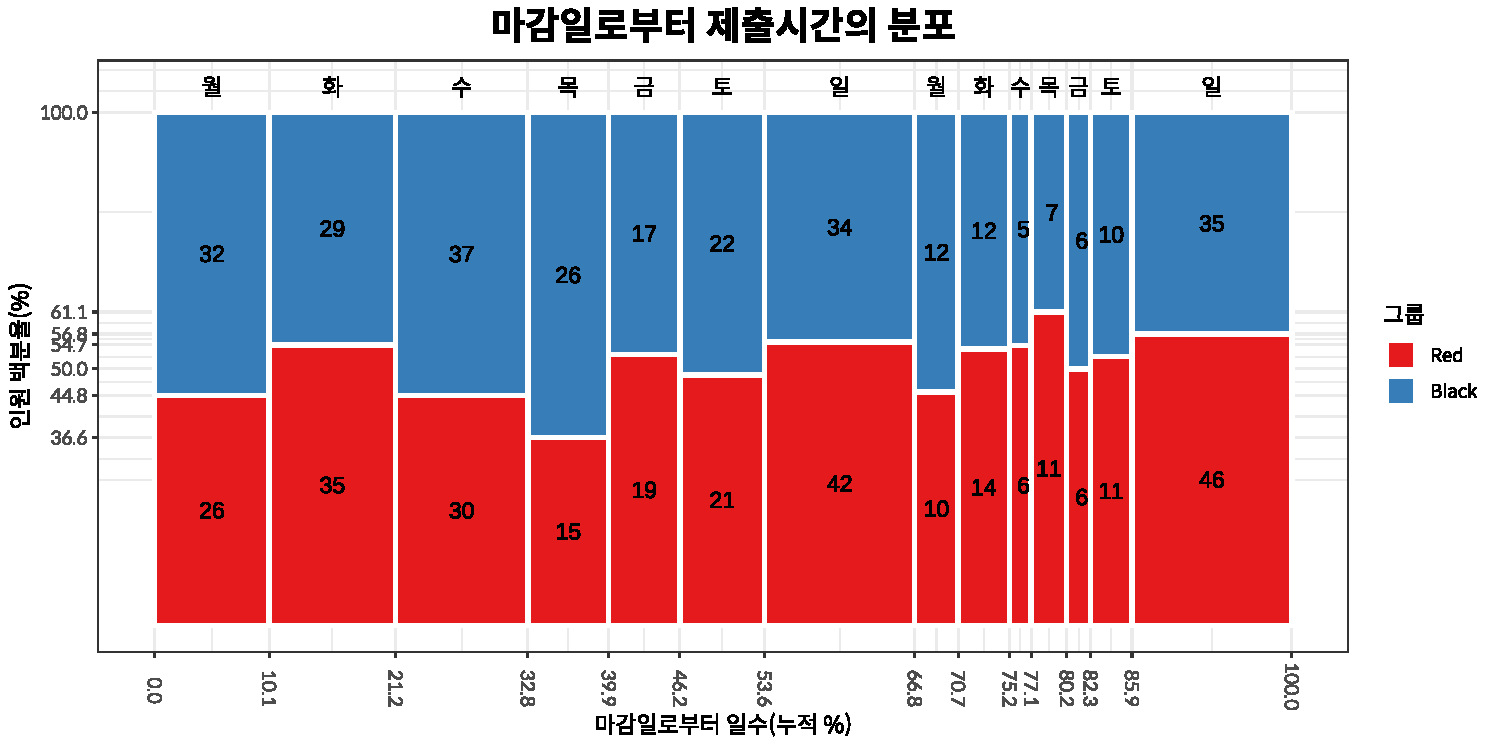
\includegraphics{quiz250303_Report_v7_files/figure-latex/unnamed-chunk-10-1.pdf}

\end{document}
